\chapter{Generating Test Cases}\label{ch:tests}

In this chapter we show how to use \tinytodo{concurrent rules and} occurrence graph grammars described in previous chapters to generate \tinytodo{test contracts and} test cases from graph grammars. In theory, these techniques can be used for any graph grammar, however we will use in the examples grammars that were generated according to the methodology presented in \cite{Junior2015} and \cite{BezerraWEIT2016}. This methodology is a systematic computer-aided way to extract graph grammars from use
cases and other text-based requirement documents.

\section{Overview of the original methodology}


\begin{figure}[!ht]
  \centering
  \fbox{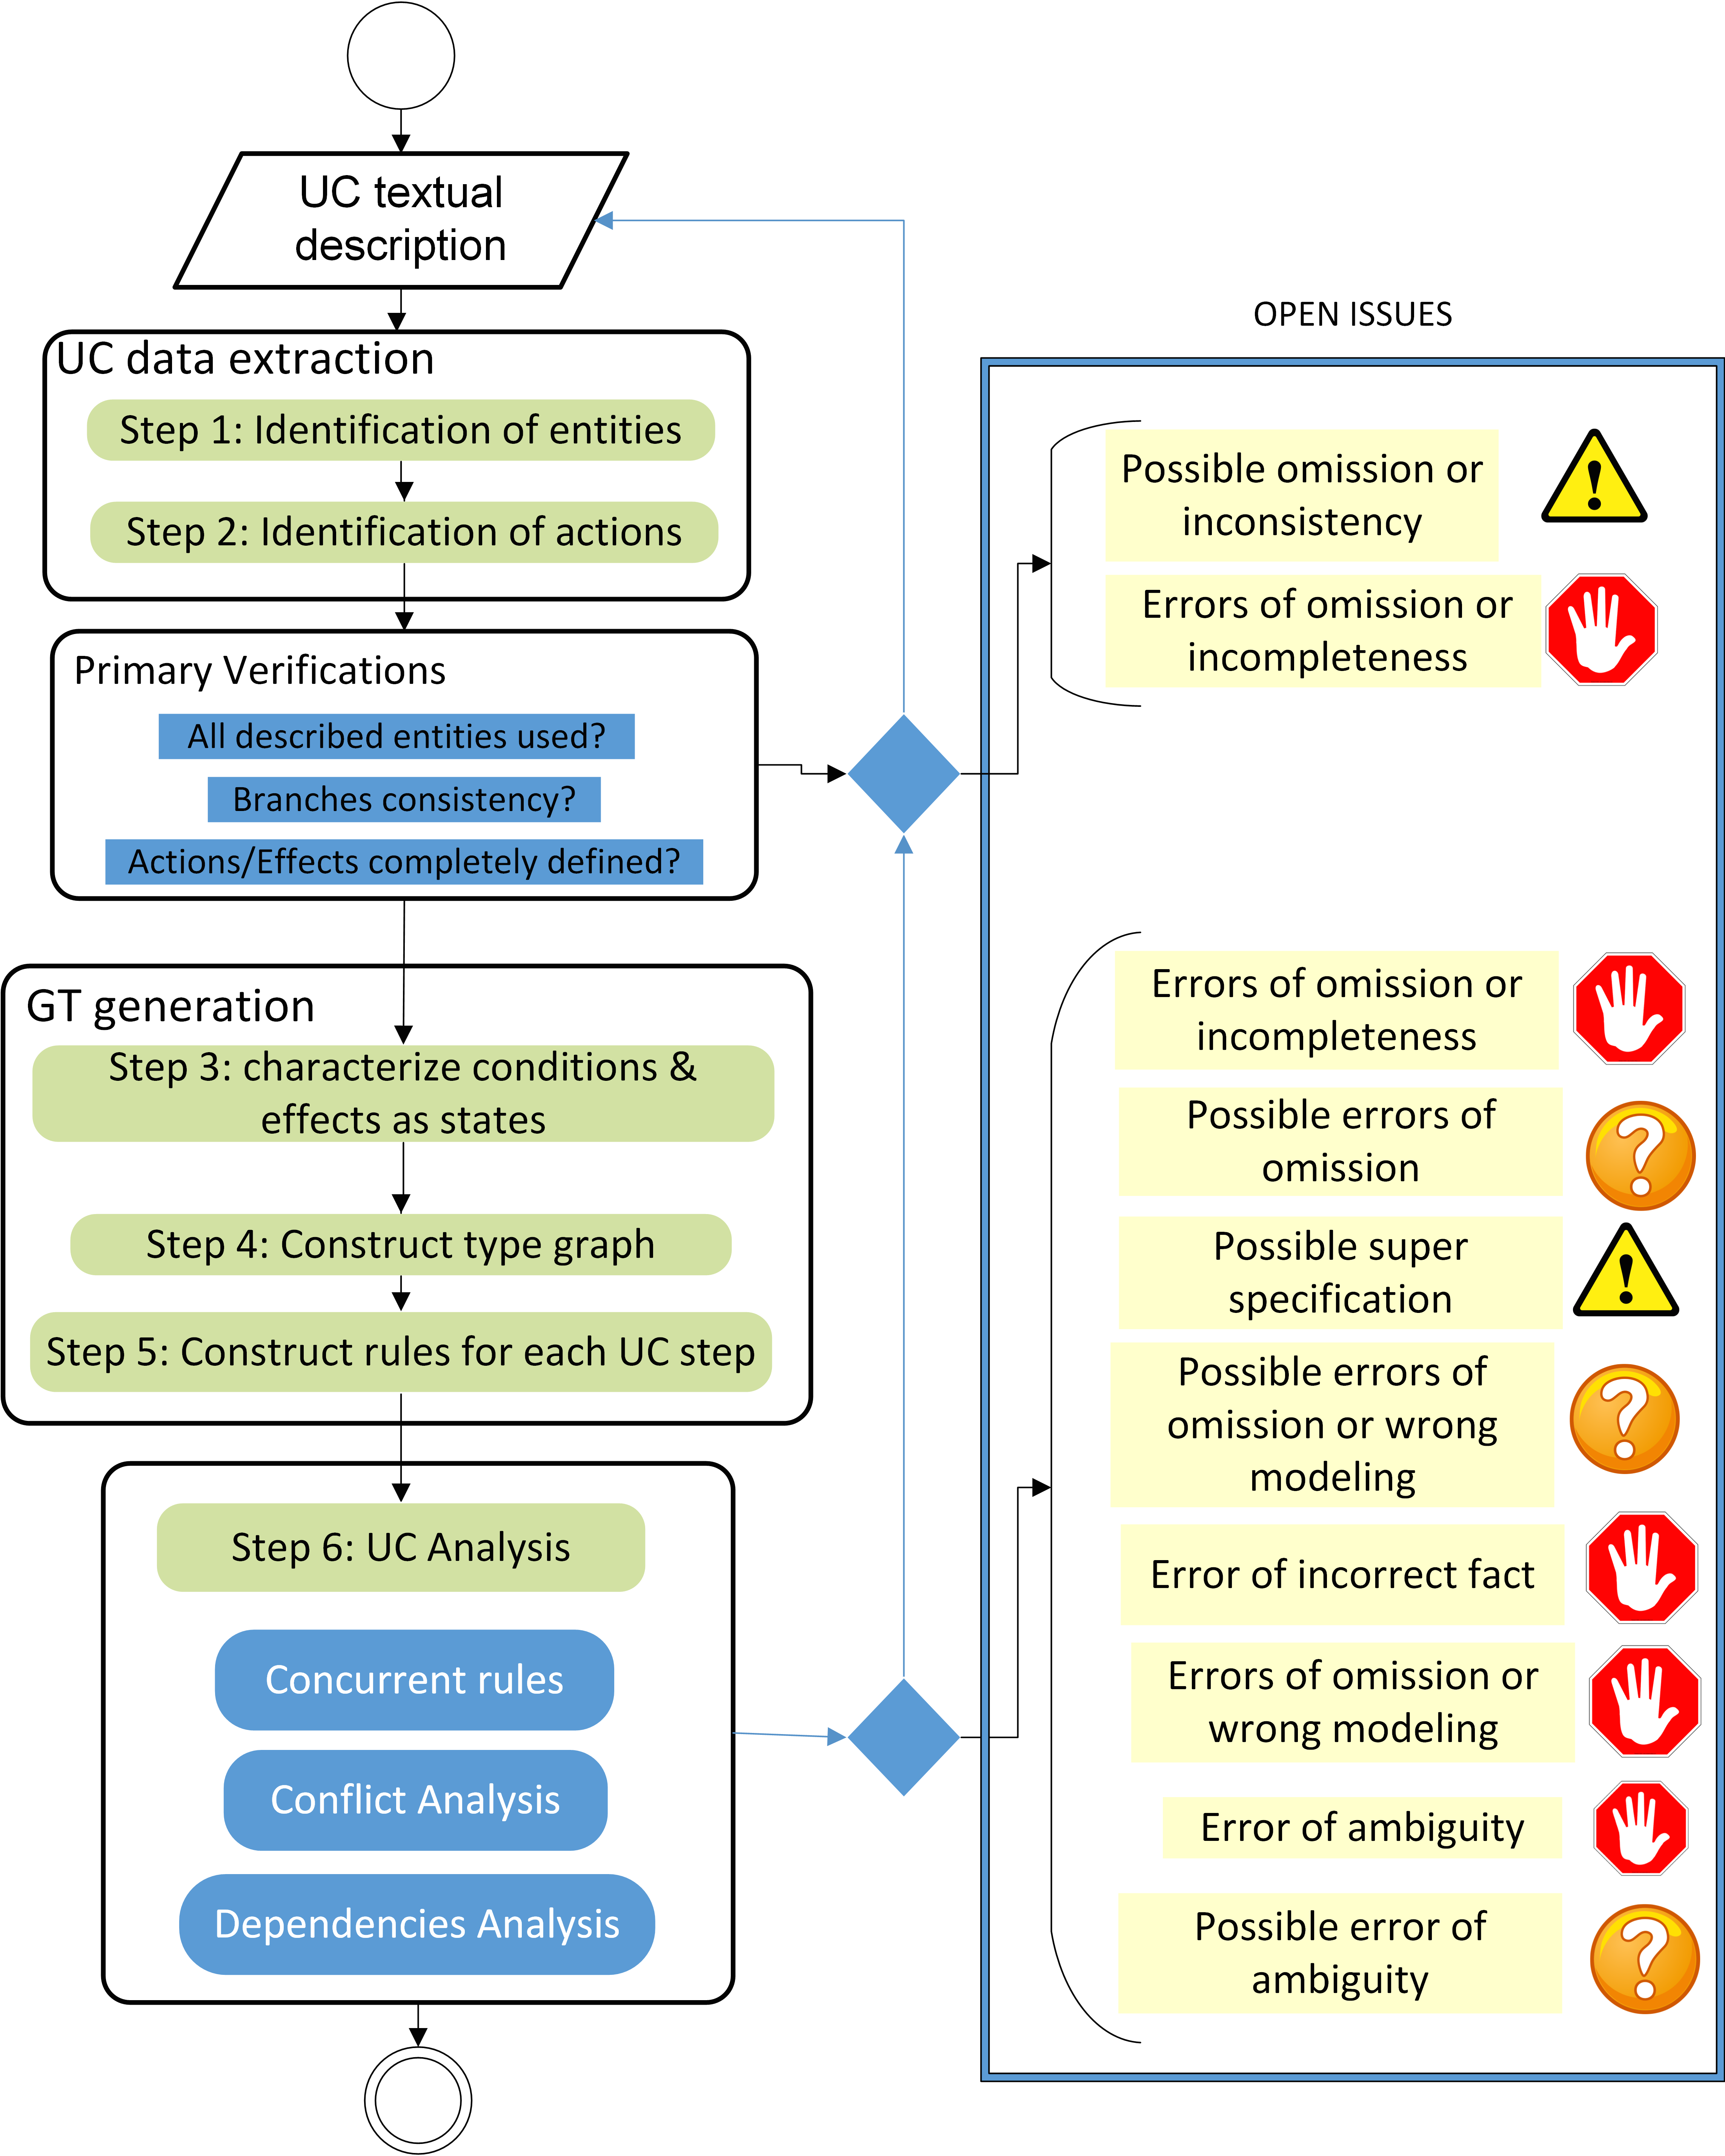
\includegraphics[scale=0.6]{images/generating-tests/methodology}}
  \caption{Overview of the methodology~\cite{Junior2015}.}\label{fig:process:doubly-typed-graph}
\end{figure}

\section{Calculating Graph Process}

\begin{itemize}
\item set of steps (rules)
\item set of sequences
\item in and out relations
\end{itemize}

We want to generate:

\begin{itemize}
\item conflict relation between the rules, presenting the conflict items and the type of the conflict.
\item dependency relation between the rules, presenting the dependency items as well as the type of the dependency.
\end{itemize}
\begin{definition}[Colimit construction]
\end{definition}

\section{Analysis and Test Generation}





